%!TEX spellcheck
%%%%%%%%%%%%%%%%%%%%%%%%%%%%%%%%%%%%%%%%%
% Beamer Presentation
% LaTeX Template
% Version 2.0 (March 8, 2022)
%
% This template originates from:
% https://www.LaTeXTemplates.com
%
% Author:
% Vel (vel@latextemplates.com)
%
% License:
% CC BY-NC-SA 4.0 (https://creativecommons.org/licenses/by-nc-sa/4.0/)
%
%%%%%%%%%%%%%%%%%%%%%%%%%%%%%%%%%%%%%%%%%

%----------------------------------------------------------------------------------------
%	PACKAGES AND OTHER DOCUMENT CONFIGURATIONS
%----------------------------------------------------------------------------------------

\documentclass[
	11pt, % Set the default font size, options include: 8pt, 9pt, 10pt, 11pt, 12pt, 14pt, 17pt, 20pt
	%t, % Uncomment to vertically align all slide content to the top of the slide, rather than the default centered
	%aspectratio=169, % Uncomment to set the aspect ratio to a 16:9 ratio which matches the aspect ratio of 1080p and 4K screens and projectors
	handout,
]{beamer}

\graphicspath{{Images/}{./}} % Specifies where to look for included images (trailing slash required)

\usepackage{booktabs} % Allows the use of \toprule, \midrule and \bottomrule for better rules in tables

%----------------------------------------------------------------------------------------
%	SELECT LAYOUT THEME
%----------------------------------------------------------------------------------------

% Beamer comes with a number of default layout themes which change the colors and layouts of slides. Below is a list of all themes available, uncomment each in turn to see what they look like.

%\usetheme{default}
%\usetheme{AnnArbor}
%\usetheme{Antibes}
%\usetheme{Bergen}
%\usetheme{Berkeley}
%\usetheme{Berlin}
%\usetheme{Boadilla}
%\usetheme{CambridgeUS}
%\usetheme{Copenhagen}
%\usetheme{Darmstadt}
%\usetheme{Dresden}
%\usetheme{Frankfurt}
%\usetheme{Goettingen}
%\usetheme{Hannover}
%\usetheme{Ilmenau}
%\usetheme{JuanLesPins}
%\usetheme{Luebeck}
\usetheme{Madrid}
%\usetheme{Malmoe}
%\usetheme{Marburg}
%\usetheme{Montpellier}
%\usetheme{PaloAlto}
%\usetheme{Pittsburgh}
%\usetheme{Rochester}
%\usetheme{Singapore}
%\usetheme{Szeged}
%\usetheme{Warsaw}

%----------------------------------------------------------------------------------------
%	SELECT COLOR THEME
%----------------------------------------------------------------------------------------

% Beamer comes with a number of color themes that can be applied to any layout theme to change its colors. Uncomment each of these in turn to see how they change the colors of your selected layout theme.

%\usecolortheme{albatross}
%\usecolortheme{beaver}
%\usecolortheme{beetle}
%\usecolortheme{crane}
%\usecolortheme{dolphin}
%\usecolortheme{dove}
%\usecolortheme{fly}
%\usecolortheme{lily}
%\usecolortheme{monarca}
%\usecolortheme{seagull}
%\usecolortheme{seahorse}
%\usecolortheme{spruce}
%\usecolortheme{whale}
%\usecolortheme{wolverine}

%----------------------------------------------------------------------------------------
%	SELECT FONT THEME & FONTS
%----------------------------------------------------------------------------------------

% Beamer comes with several font themes to easily change the fonts used in various parts of the presentation. Review the comments beside each one to decide if you would like to use it. Note that additional options can be specified for several of these font themes, consult the beamer documentation for more information.

\usefonttheme{default} % Typeset using the default sans serif font
%\usefonttheme{serif} % Typeset using the default serif font (make sure a sans font isn't being set as the default font if you use this option!)
%\usefonttheme{structurebold} % Typeset important structure text (titles, headlines, footlines, sidebar, etc) in bold
%\usefonttheme{structureitalicserif} % Typeset important structure text (titles, headlines, footlines, sidebar, etc) in italic serif
%\usefonttheme{structuresmallcapsserif} % Typeset important structure text (titles, headlines, footlines, sidebar, etc) in small caps serif

%------------------------------------------------

%\usepackage{mathptmx} % Use the Times font for serif text
\usepackage{palatino} % Use the Palatino font for serif text
\usepackage{hyperref}
%\usepackage{helvet} % Use the Helvetica font for sans serif text
\usepackage[default]{opensans} % Use the Open Sans font for sans serif text
%\usepackage[default]{FiraSans} % Use the Fira Sans font for sans serif text
%\usepackage[default]{lato} % Use the Lato font for sans serif text
\usepackage{ctex}


%----------------------------------------------------------------------------------------
%	SELECT INNER THEME
%----------------------------------------------------------------------------------------

% Inner themes change the styling of internal slide elements, for example: bullet points, blocks, bibliography entries, title pages, theorems, etc. Uncomment each theme in turn to see what changes it makes to your presentation.

%\useinnertheme{default}
\useinnertheme{circles}
%\useinnertheme{rectangles}
%\useinnertheme{rounded}
%\useinnertheme{inmargin}

%----------------------------------------------------------------------------------------
%	SELECT OUTER THEME
%----------------------------------------------------------------------------------------

% Outer themes change the overall layout of slides, such as: header and footer lines, sidebars and slide titles. Uncomment each theme in turn to see what changes it makes to your presentation.

%\useoutertheme{default}
%\useoutertheme{infolines}
%\useoutertheme{miniframes}
%\useoutertheme{smoothbars}
%\useoutertheme{sidebar}
%\useoutertheme{split}
%\useoutertheme{shadow}
%\useoutertheme{tree}
%\useoutertheme{smoothtree}

%\setbeamertemplate{footline} % Uncomment this line to remove the footer line in all slides
%\setbeamertemplate{footline}[page number] % Uncomment this line to replace the footer line in all slides with a simple slide count

%\setbeamertemplate{navigation symbols}{} % Uncomment this line to remove the navigation symbols from the bottom of all slides

%----------------------------------------------------------------------------------------
%	PRESENTATION INFORMATION
%----------------------------------------------------------------------------------------

\title[Geometry]{Geometry} % The short title in the optional parameter appears at the bottom of every slide, the full title in the main parameter is only on the title page

\subtitle{几何} % Presentation subtitle, remove this command if a subtitle isn't required

\author[张凡]{张凡} % Presenter name(s), the optional parameter can contain a shortened version to appear on the bottom of every slide, while the main parameter will appear on the title slide

\institute[XDF]{新东方国际教育 \\ \smallskip \textit{zhangfan@xdf.cn}} % Your institution, the optional parameter can be used for the institution shorthand and will appear on the bottom of every slide after author names, while the required parameter is used on the title slide and can include your email address or additional information on separate lines

\date[\today]{GRE 冲分班数学 \\ \today} % Presentation date or conference/meeting name, the optional parameter can contain a shortened version to appear on the bottom of every slide, while the required parameter value is output to the title slide

%----------------------------------------------------------------------------------------


%----------------------------------------------------------------------------------------
%	Section Slide
%----------------------------------------------------------------------------------------
\AtBeginSection[]{
  \begin{frame}
  \vfill
  \centering
  \begin{beamercolorbox}[sep=8pt,center,shadow=true,rounded=true]{title}
    \usebeamerfont{title}\insertsectionhead\par%
  \end{beamercolorbox}
  \vfill
  \end{frame}

%----------------------------------------------------------------------------------------
%	TABLE OF CONTENTS SLIDE OF THE CURRENT SECTION
%----------------------------------------------------------------------------------------
	\begin{frame}
		\frametitle{Presentation Overview for \secname} % Slide title, remove this command for no title
		\tableofcontents[currentsection, hideothersubsections, sectionstyle=show/show]
	\end{frame}
  }

%----------------------------------------------------------------------------------------

\AtBeginSubsection[]{
  \begin{frame}
  \vfill
  \centering
    \usebeamerfont{title}\insertsubsectionhead\par%
  \vfill
  \end{frame}
}
%----------------------------------------------------------------------------------------


\begin{document}

%----------------------------------------------------------------------------------------
%	TITLE SLIDE
%----------------------------------------------------------------------------------------

\begin{frame}
	\titlepage % Output the title slide, automatically created using the text entered in the PRESENTATION INFORMATION block above
\end{frame}



%----------------------------------------------------------------------------------------
%	PRESENTATION BODY SLIDES
%----------------------------------------------------------------------------------------
\begin{frame}
	\frametitle{To Begin With} % Slide title, remove this command for no title

	\begin{block}{QR Mathematical Convention 3}
		All figures are assumed to lie in a plane unless otherwise indicated.
	\end{block}

		\begin{block}{QR Mathematical Convention 4}
		Geometric figures are not necessarily drawn to scale.
	\end{block}
	\begin{example}
		\begin{itemize}
			\item \alert{Can not} assume  that quantities such as lengths and  are as they appear in a figure
			\item \alert{Can not} assume  that angle measures such as lengths and  are as they appear in a figure 
			\item \alert{Can} assume all geometric objects are in the relative positions shown.
		\end{itemize}
	\end{example}
\end{frame}

%------------------------------------------------

\begin{frame}
	\frametitle{Rely on Your Geometric Reasoning, not Estimating or Comparing Quantities By Eyesight} % Slide title, remove this command for no title
	\framesubtitle{用几何推理做题!}
	\begin{columns}[t] 
		\begin{column}{0.4\textwidth} % Left column width
		Which of the following statements \alert{Must Be} right?
			\begin{figure}
				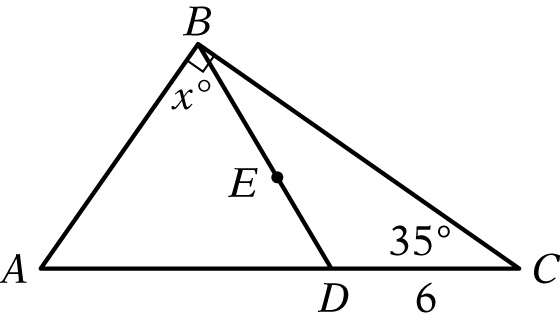
\includegraphics[width=\linewidth]{Not_Scale.jpg}
			\end{figure}
		\end{column}

	\begin{column}{0.6\textwidth} % Right column width
	\begin{enumerate}
		\item Points $A$, $D$, and $C$ are distinct. Point $D$ lies between points $A$ and $C$, and the line containing them is straight.
		\item The length of line segment $AD$ is less than the length of line segment $AC$.
		\item $ABC,\ ABD,\ $ and $DBC$ are triangles.
		\item Point $E$ lies on line segment $BD$.
		\item Angle $ABC$ is a right angle, as indicated by the small square symbol at point $B$.
		\item The length of line segment $DC$ is 6, and the measure of angle $C$ is 35 degrees.
		\item The measure of angle $ABD$ is x degrees, and $x<90$.
	\end{enumerate}
	\end{column}
	\end{columns}
\end{frame}

%------------------------------------------------

\begin{frame}
	\frametitle{Rely on Your Geometric Reasoning, not Estimating or Comparing Quantities By Eyesight} % Slide title, remove this command for no title
	\framesubtitle{用几何推理做题!}
	\begin{columns}[t] 
		\begin{column}{0.4\textwidth} % Left column width
		Which of the following statements \alert{Must Be} right?
			\begin{figure}
				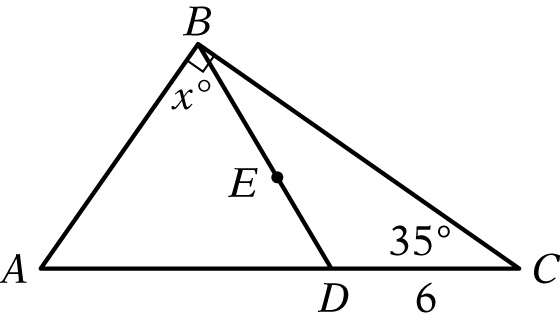
\includegraphics[width=\linewidth]{Not_Scale.jpg}
			\end{figure}
				Answer: \textbf{\alert{They all must be right!}}
		\end{column}

	\begin{column}{0.6\textwidth} % Right column width
	\begin{enumerate}
		\item Points $A$, $D$, and $C$ are distinct. Point D lies between points $A$ and $C$, and the line containing them is straight.
		\item The length of line segment $AD$ is less than the length of line segment $AC$.
		\item $ABC,\ ABD,\ $ and $DBC$ are triangles.
		\item Point $E$ lies on line segment $BD$.
		\item Angle $ABC$ is a right angle, as indicated by the small square symbol at point $B$.
		\item The length of line segment $DC$ is 6, and the measure of angle $C$ is 35 degrees.
		\item The measure of angle $ABD$ is x degrees, and $x<90$.
	\end{enumerate}
	\end{column}
	\end{columns}
\end{frame}

%------------------------------------------------

\begin{frame}
	\frametitle{Rely on Your Geometric Reasoning, not Estimating or Comparing Quantities By eyesight} % Slide title, remove this command for no title
	\framesubtitle{用几何推理做题!}
	\begin{columns}[t] 
		\begin{column}{0.4\textwidth} % Left column width
		Which of the following statements \alert{Must Be} right?
			\begin{figure}
				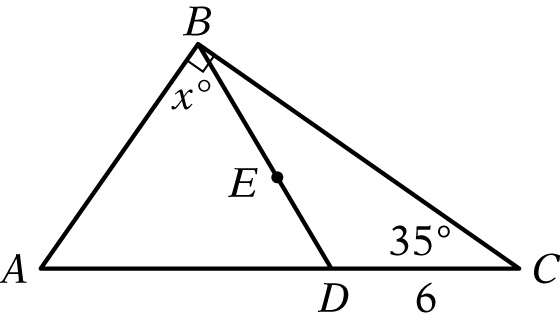
\includegraphics[width=\linewidth]{Not_Scale.jpg}
			\end{figure}
		\end{column}

	\begin{column}{0.6\textwidth} % Right column width
	\begin{enumerate}
		\item The length of line segment $AD$ is greater than the length of line segment $DC$.
		\item The measures of angles $BAD$ and $BDA$ are equal.
		\item The measure of angle is less than x degrees.
		\item The area of triangle $ABD$ is greater than the area of triangle $DBC$.
	\end{enumerate}
	\pause
	Answer: \textbf{\alert{They are all not necessarily right!}}
	\end{column}
	\end{columns}
\end{frame}

%------------------------------------------------

% vertices raddii plura

%------------------------------------------------

\section{Lines and Angles}

%------------------------------------------------

\subsection{Lines}

%------------------------------------------------

\begin{frame}
	\frametitle{Congruent line segments} % Slide title, remove this command for no title
	\framesubtitle{全等线段}
	\framesubtitle{用几何推理做题!}
		\begin{figure}
			\includegraphics[width=\linewidth]{Lines.jpg}
			\caption{$BC$ and $CD$ are congruent line segments.}
		\end{figure}

		\begin{definition}
		Line segments that have equal lengths are called \alert{congruent line segments} .
		\end{definition}
\end{frame}

%------------------------------------------------

\begin{frame}
	\frametitle{Math Vocab!} % Slide title, remove this command for no title
	\framesubtitle{专业名词记忆时间!}
	
	{\Huge congruent}\\
	{\LARGE /kənˈɡro͞oənt,ˈkäNGɡro͞oənt/\\
		\bigskip\bigskip
	(of figures) identical in form; coinciding exactly when superimposed. \\ 
	全等:相同,叠加的时候完全重合}

\end{frame}

%------------------------------------------------


%------------------------------------------------

\subsection{Angles}

%------------------------------------------------

\begin{frame}
	\frametitle{Opposite Angles} % Slide title, remove this command for no title
	\framesubtitle{对角相等}
	\begin{columns}[t] 
		\begin{column}{0.4\textwidth} % Left column width
			\begin{figure}
				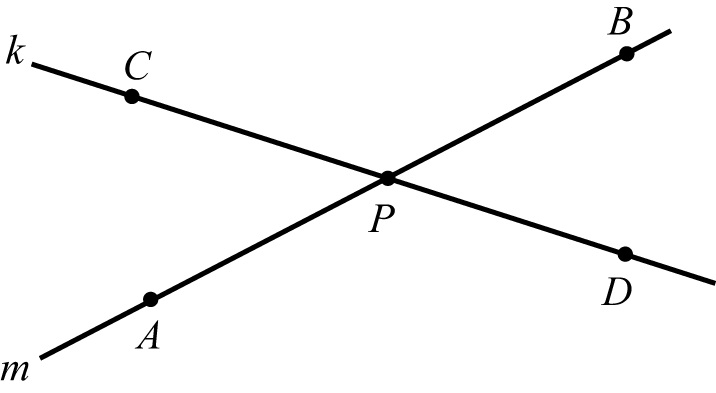
\includegraphics[width=\linewidth]{Angles.jpg}
				\caption{$\angle APC$ and $\angle BPD$ are opposite angles; So are  $\angle CPB$ and $\angle DPA$.}
			\end{figure}
		\end{column}

	\begin{column}{0.6\textwidth} % Right column width
		\begin{definition}
		Opposite angles have equal measure, and angles that have equal measure are called congruent angles. Hence, \alert{opposite angles are congruent}.
		\end{definition}
	\end{column}
	\end{columns}
\end{frame}

%------------------------------------------------

\begin{frame}
	\frametitle{Acute,Right, Obtuse Angles} % Slide title, remove this command for no title
	\framesubtitle{锐角\ 直角\ 钝角}

		\begin{figure}
			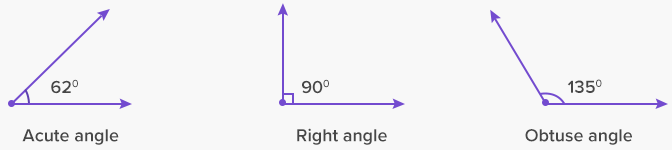
\includegraphics[width=\linewidth]{Acute_Right_Obtuse.png}
			\caption{$BC$ and $CD$ are congruent line segments.}
		\end{figure}

		\begin{definition}
		\begin{itemize}
			\item An angle with measure less than 90° is called an \alert{acute angle}.
			\item An angle with a measure of 90° is called a \alert{right angle}.
			\item an angle with measure between 90° and 180° is called an \alert{obtuse angle}.
		\end{itemize}
		\end{definition}
\end{frame}

%------------------------------------------------

\subsection{Parallel Lines}

%------------------------------------------------

\begin{frame}
	\frametitle{Parallel Lines} % Slide title, remove this command for no title
	\framesubtitle{平行线同位角相等,内错角之和为180度}
		\begin{figure}
			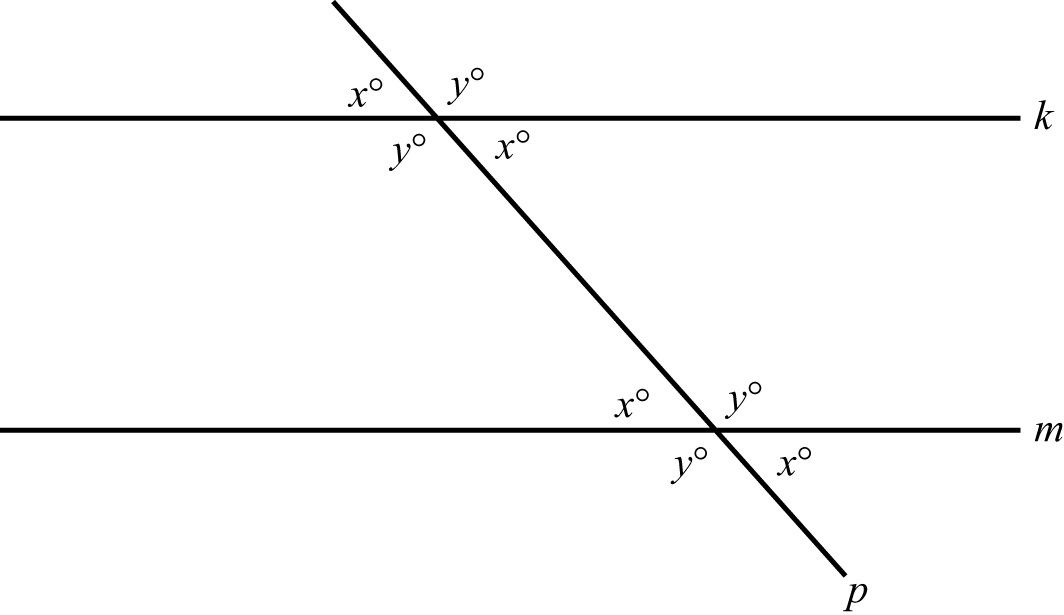
\includegraphics[width=0.9\linewidth]{Parallel_Lines.jpg}
			\caption{$k \parallel m$}
		\end{figure}
\end{frame}

%------------------------------------------------

\section{Triangles}

%------------------------------------------------

\subsection{Equilateral Triangles}

%------------------------------------------------

\begin{frame}
	\frametitle{Math Vocab!} % Slide title, remove this command for no title
	\framesubtitle{专业名词记忆时间!}
	
	{\Huge Equilateral}\\
	{\LARGE /ˌēkwəˈladərəl,ˌekwəˈladərəl/\\
		\bigskip\bigskip
	(of figures) having all its sides of the same length.. \\ 
	等边:所有边长相等}

\end{frame}

%------------------------------------------------

\begin{frame}
	\frametitle{Equilateral Triangles} % Slide title, remove this command for no title
	\framesubtitle{等边三角形:内角均为60度}

		\begin{figure}
			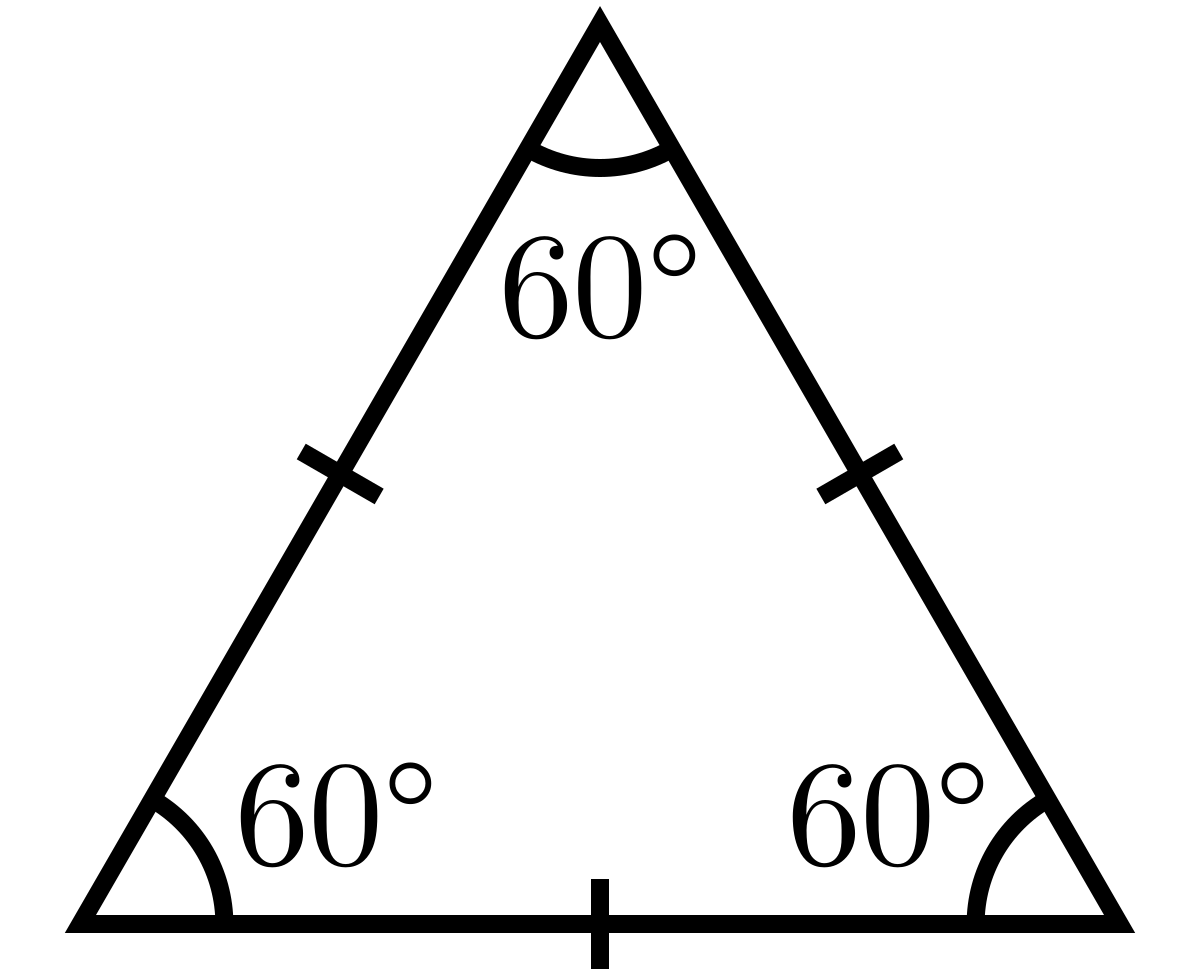
\includegraphics[width=0.6\linewidth]{Triangle.Equilateral.svg.png}
			\caption{The measures of the three interior angles of such a triangle are
equal, and each measure is 60°.}
		\end{figure}
\end{frame}

%------------------------------------------------

\subsection{Isosceles Triangles}

%------------------------------------------------

\begin{frame}
	\frametitle{Math Vocab!} % Slide title, remove this command for no title
	\framesubtitle{专业名词记忆时间!}
	
	{\Huge Isosceles}\\
	{\LARGE /īˈsäsəˌlēz/\\
		\bigskip\bigskip
	(of a triangle) having two sides of equal length. \\ 
	等腰三角形:两边长相等}

\end{frame}

%------------------------------------------------

\begin{frame}
	\frametitle{Isosceles Triangles} % Slide title, remove this command for no title
	\framesubtitle{等腰三角形:内角均为60度}



	\begin{columns}[t] 

		\begin{column}{0.5\textwidth} % Left column width
			\begin{figure}
				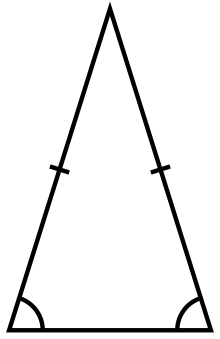
\includegraphics[width=0.6\linewidth]{220px-Triangle.Isosceles.svg.png}
				\caption{Congruent sides suggest congruent angles.}
			\end{figure}		
		\end{column}
		\begin{column}{0.5\textwidth} % Right column width
		\begin{theorem}[两角相等互推两边相等]
			If a triangle has two congruent sides, then the angles opposite
the two congruent sides are congruent. \alert{The converse is also true}.
		\end{theorem}
		\pause
		\begin{theorem}[Law Of Sines\ 正弦定理]
			\begin{equation*}
				\frac{\sin A}{a}=\frac{\sin B}{b}=\frac{\sin C}{c}
			\end{equation*}
		\end{theorem}
		\end{column}
	\end{columns}
\end{frame}

%------------------------------------------------

\subsection{The Right Triangles}

%------------------------------------------------

\begin{frame}
	\frametitle{Math Vocab!} % Slide title, remove this command for no title
	\framesubtitle{专业名词记忆时间!}
	
	\begin{columns}[t] 
		\begin{column}{0.7\textwidth} % Left column width
			{\Huge hypotenuse}\\
	{\LARGE /hīˈpätnˌ(y)o͞os/\\
		\bigskip\bigskip
	the longest side of a right triangle, opposite the right angle. \\ 
	斜边:直角三角形直角对边}
	\bigskip\bigskip\bigskip\bigskip

		{\Huge leg}\\{\LARGE 直角边}
		\end{column}
		\begin{column}{0.3\textwidth} % Right column width
					\begin{figure}
				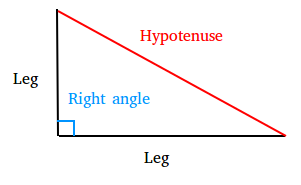
\includegraphics[width=\linewidth]{Hypotenuse.png}
			\end{figure}	
		\end{column}
	\end{columns}
\end{frame}

%------------------------------------------------

\begin{frame}
	\frametitle{The Pythagorean Theorem} % Slide title, remove this command for no title
	\framesubtitle{勾股定理}
	\begin{figure}
		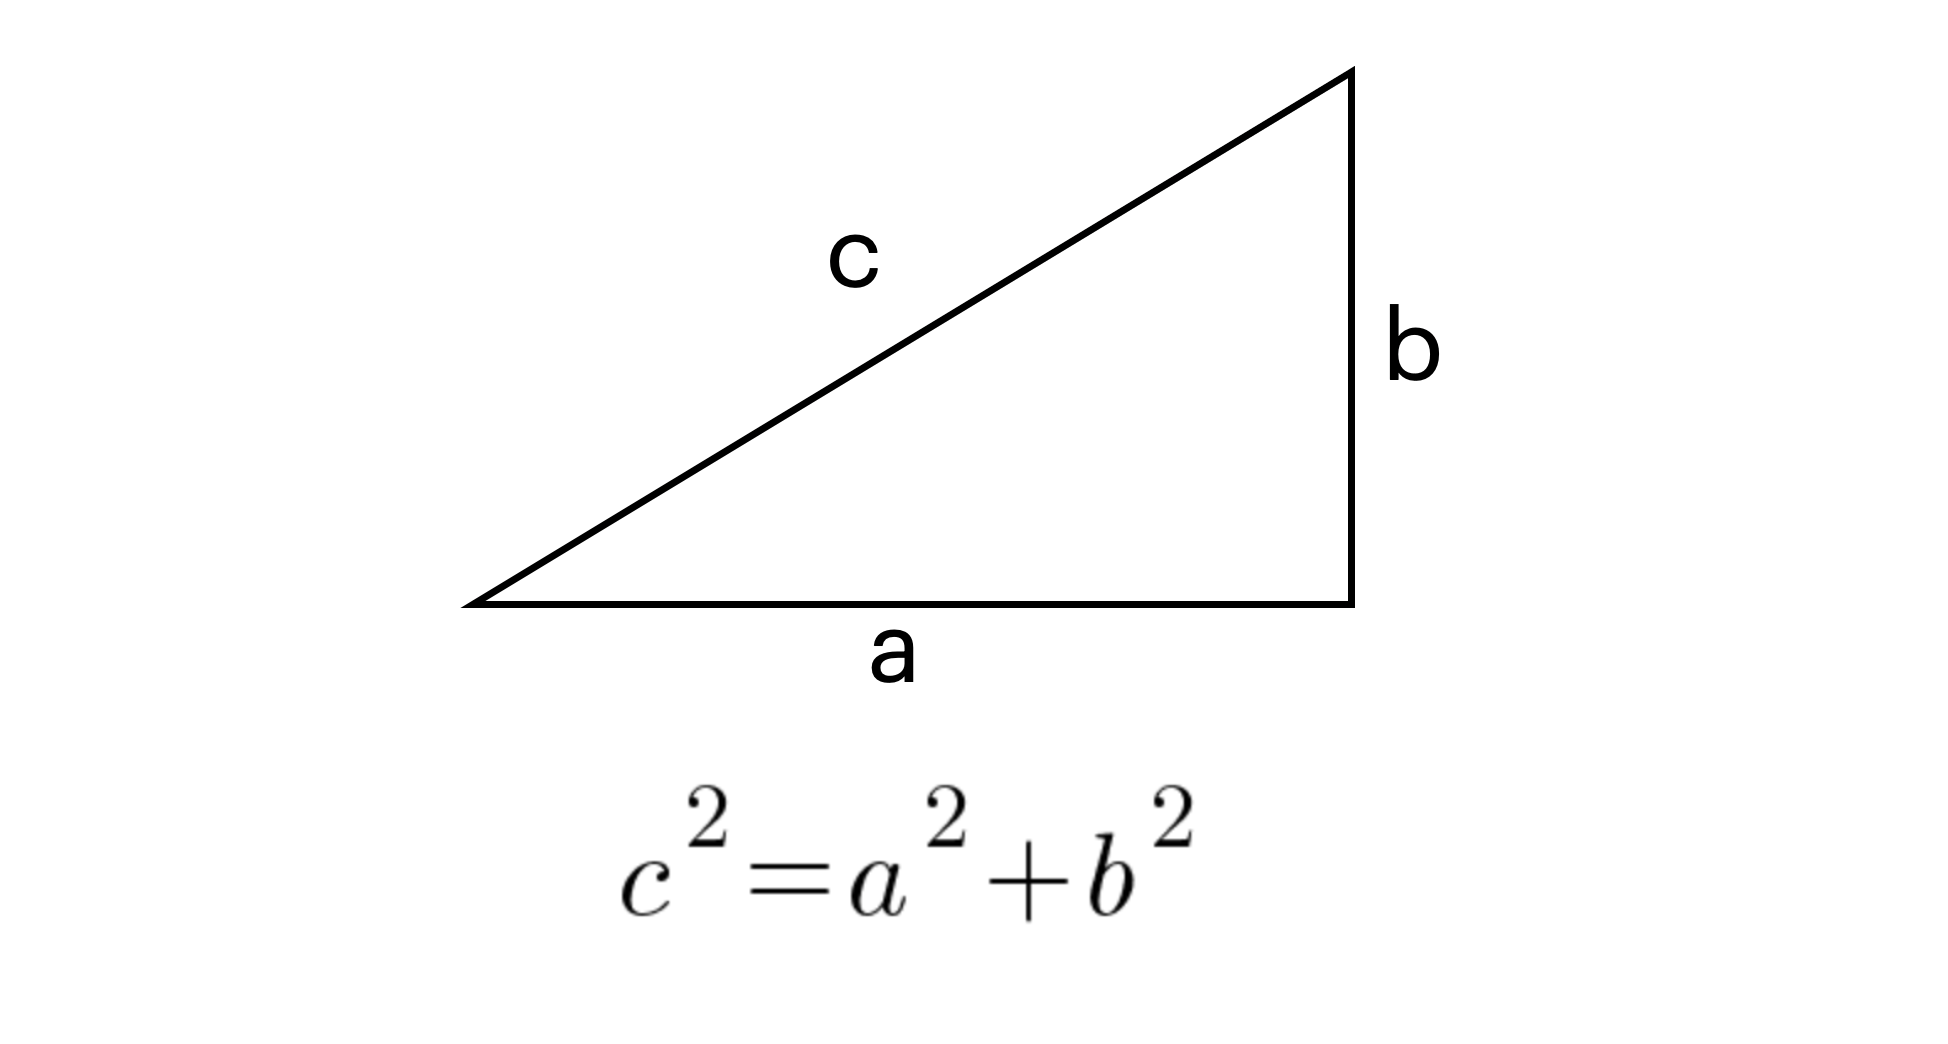
\includegraphics[width=\linewidth]{Pythagorean.png}
	\end{figure}	
\end{frame}

%------------------------------------------------

\begin{frame}
	\frametitle{Math Vocab!} % Slide title, remove this command for no title
	\framesubtitle{专业名词记忆时间!}
	
	{\Huge Pythagorean}\\
	{\LARGE /īˈsäsəˌlēz/\\
		\bigskip\bigskip
	relating to or characteristic of the Greek philosopher Pythagoras or his ideas. \\ 
	毕达哥拉斯}
\end{frame}

%------------------------------------------------

\begin{frame}
	\frametitle{45°-45°-90° Triangle} % Slide title, remove this command for no title
	\framesubtitle{边长比为1:1:$\sqrt{2}$}
	\begin{figure}
		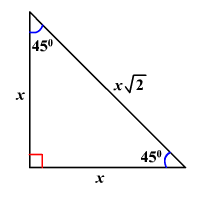
\includegraphics[width=0.5\linewidth]{45-45-90-Triangle.png}
		\caption{\alert{Isosceles Right Triangle}}
	\end{figure}	
\end{frame}

%------------------------------------------------


\begin{frame}
	\frametitle{30°-60°-90° Triangle} % Slide title, remove this command for no title
	\framesubtitle{边长比为1:$\sqrt{3}$:2}
	\begin{figure}
		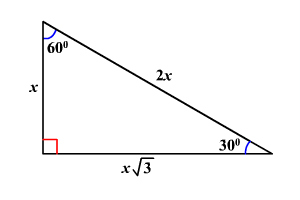
\includegraphics[width=0.5\linewidth]{30_60_90_triangle.png}
	\end{figure}	
\end{frame}


%------------------------------------------------

\begin{frame}
	\frametitle{The Triangle Inequalities} % Slide title, remove this command for no title
	\framesubtitle{三角不等式}
	\begin{theorem}[两边之和大于第三边;两边之差小于第三边]
		\begin{equation*}
			\begin{aligned}
				&a-b<c<a+b 
			\end{aligned}
		\end{equation*}
	\end{theorem}
\end{frame}


%------------------------------------------------


\begin{frame}
	\frametitle{Exterior Angle of Triangles} % Slide title, remove this command for no title
	\framesubtitle{外角等于相对应内对角之和}
		\begin{figure}
		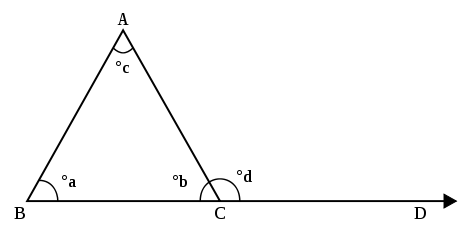
\includegraphics[width=0.5\linewidth]{Exterio_Angle.png}
	\end{figure}	
	\begin{theorem}
		\begin{equation*}
				d = a + c		
		\end{equation*}
	\end{theorem}
\end{frame}


%------------------------------------------------

\subsection{The Area of a Triangle}

%------------------------------------------------

\begin{frame}
	\frametitle{The Area of a Triangle} % Slide title, remove this command for no title
	\framesubtitle{底乘高除以二}
	\begin{figure}
		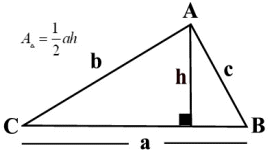
\includegraphics[width=0.5\linewidth]{Area_Triangle.png}
	\end{figure}	
\end{frame}

%------------------------------------------------

\subsection{Congruent Triangles}

%------------------------------------------------

\begin{frame}
	\frametitle{SSS, SAS, ASA Congruence} % Slide title, remove this command for no title
	\framesubtitle{边边边\ 边角边\ 角边角\ 全等}
			\begin{theorem}[Side-Side-Side Congruence]
				If the three sides of one triangle are congruent to the three
sides of another triangle, then the triangles are congruent.
			\end{theorem}

			\begin{theorem}[Side-Angle-Side Congruence]
				If two sides and the included angle of one triangle are
congruent to two sides and the included angle of another triangle,
then the triangles are congruent.
			\end{theorem}

			\begin{theorem}[Angle-Side-Angle Congruence]
				If two angles and the included side of one triangle are
congruent to two angles and the included side of another triangle,
then the triangles are congruent.
			\end{theorem}
What about AAS?\pause \alert{\textbf{Yes!}}
\end{frame}

%------------------------------------------------

\subsection{Similar Triangles}

%------------------------------------------------

\begin{frame}
	\frametitle{Scale Factor Of Similarity} % Slide title, remove this command for no title
	\framesubtitle{相似比例}
		\begin{figure}
			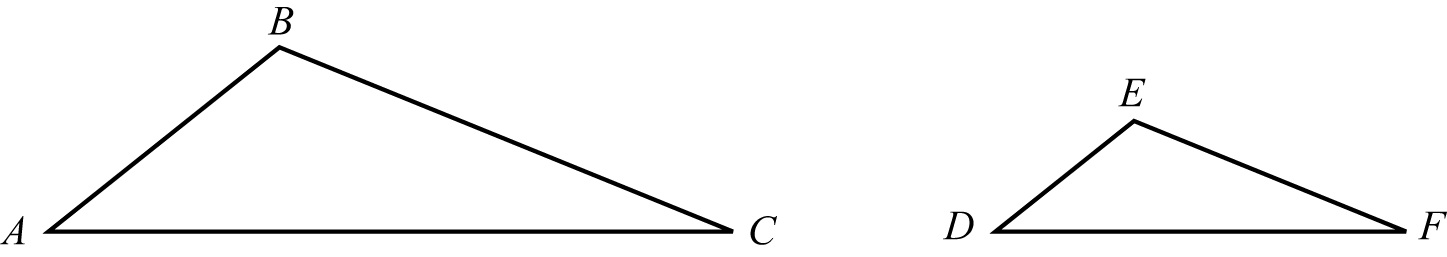
\includegraphics[width=0.8\linewidth]{Scale_Factor.jpg}
			\caption{Two similar triangles}
		\end{figure}
			\begin{definition}
				More precisely, two triangles are similar if their
vertices can be matched up so that the corresponding angles are congruent or,
equivalently, the lengths of the corresponding sides have the same ratio,
called \alert{the scale factor of similarity}.
			\end{definition}
How to prove similarity? \pause \alert{\textbf{AA!}}
\end{frame}

%------------------------------------------------

\begin{frame}
	\frametitle{Math Vocab!} % Slide title, remove this command for no title
	\framesubtitle{专业名词记忆时间!}
	
	{\Huge vertices}\\

		\bigskip\bigskip
	{\LARGE The plural noun of vertex \\ 
	顶点点的复数}

\end{frame}

%------------------------------------------------

\section{Quadrilaterals}

%------------------------------------------------

\begin{frame}
	\frametitle{Math Vocab!} % Slide title, remove this command for no title
	\framesubtitle{专业名词记忆时间!}
	
	{\Huge quadrilateral}\\
	{\LARGE /ˌkwädrəˈladərəl,ˌkwädrəˈlatrəl/\\
		\bigskip\bigskip
	a four-sided figure. \\ 
	四边形}

\end{frame}

%------------------------------------------------

\subsection{Rectangle}

%------------------------------------------------

\begin{frame}
	\frametitle{Rectangle} % Slide title, remove this command for no title
	\framesubtitle{矩形}
	\begin{definition}
		A quadrilateral with four right angles is called a rectangle.
Opposite sides of a rectangle are parallel and congruent, and the two
diagonals are also congruent. \\
A rectangle with four congruent sides is called a square.
	\end{definition}

	\begin{columns}[t] 
		\begin{column}{0.5\textwidth} % Left column width
			\begin{figure}
				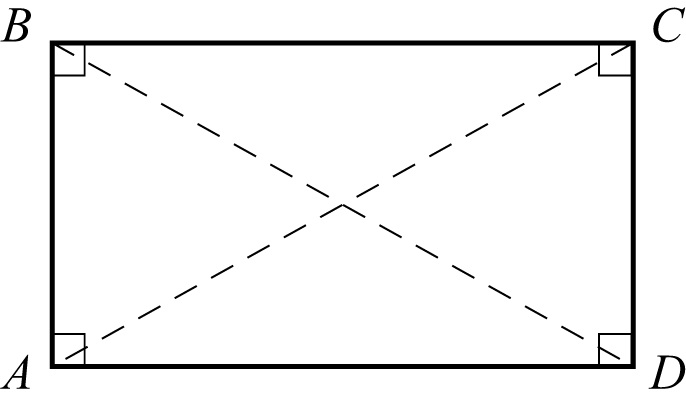
\includegraphics[width=\linewidth]{Retangle.jpg}
			\end{figure}
		\end{column}
		\begin{column}{0.5\textwidth} % Right column width
			\begin{equation*}
				Area:\ A = base \cdot height
			\end{equation*}
		\end{column}
	\end{columns}
\end{frame}

%------------------------------------------------

\subsection{Parallelogram}

%------------------------------------------------

\begin{frame}
	\frametitle{Math Vocab!} % Slide title, remove this command for no title
	\framesubtitle{专业名词记忆时间!}
	
	{\Huge parallelogram}\\
	{\LARGE /ˌperəˈleləˌɡram/\\
		\bigskip\bigskip
	a four-sided plane rectilinear figure with opposite sides parallel. \\ 
	平行四边形}

\end{frame}

%------------------------------------------------
	\begin{frame}
	\frametitle{Parallelogram} % Slide title, remove this command for no title
	\framesubtitle{平行四边形}
	\begin{definition}
		A quadrilateral in which both pairs of opposite sides are parallel
		is called a parallelogram. In a parallelogram, opposite sides are
		congruent and opposite angles are congruent. \\
		Note that all rectangles are parallelograms.
	\end{definition}

	\begin{columns}[t] 
		\begin{column}{0.5\textwidth} % Left column width
			\begin{figure}
				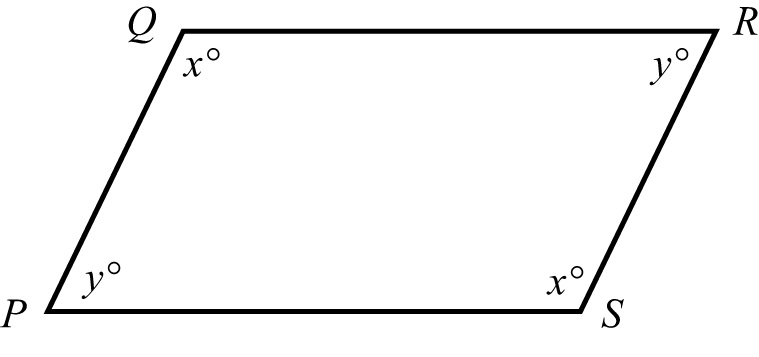
\includegraphics[width=\linewidth]{Parallelogram.jpg}
			\end{figure}
		\end{column}

		\begin{column}{0.5\textwidth} % Right column width
			\begin{equation*}
				Area:\ A = base \cdot height
			\end{equation*}
		\end{column}
	\end{columns}
\end{frame}

%------------------------------------------------

\subsection{Trapezoid}

%------------------------------------------------


\section{Polygons}

%------------------------------------------------


\section{Circles}

%------------------------------------------------

\subsection{Radius, Diameter, And Chord}

%------------------------------------------------

\subsection{Central Angle, Arc, Circumference and Area}

%------------------------------------------------

\subsection{Tangent Lines}

%------------------------------------------------

\subsection{Inscribed In Or Circumscribed About The Polygon}

%------------------------------------------------

\subsection{Concentric Circles}

%------------------------------------------------


\section{Three-Dimensional Figures}

%------------------------------------------------

\subsection{Rectangular Solid(Right Rectangular Prism)}

%------------------------------------------------

\subsection{Circular Cylinder And Right Circular Cylinder}

%------------------------------------------------

% 	\begin{columns}[t] 

% 		\begin{column}{0.5\textwidth} % Left column width
% 		\end{column}
% 		\begin{column}{0.5\textwidth} % Right column width
% 		\end{column}
% 	\end{columns}


% 	\begin{figure}
% 		
\includegraphics[width=0.8\linewidth]{creodocs_logo.pdf}
% 		\caption{Creodocs logo.}
% 	\end{figure}


% \begin{frame}
% 	\frametitle{A Real QR Problem!}
% 	\framesubtitle{}
% 	\begin{figure}
% 		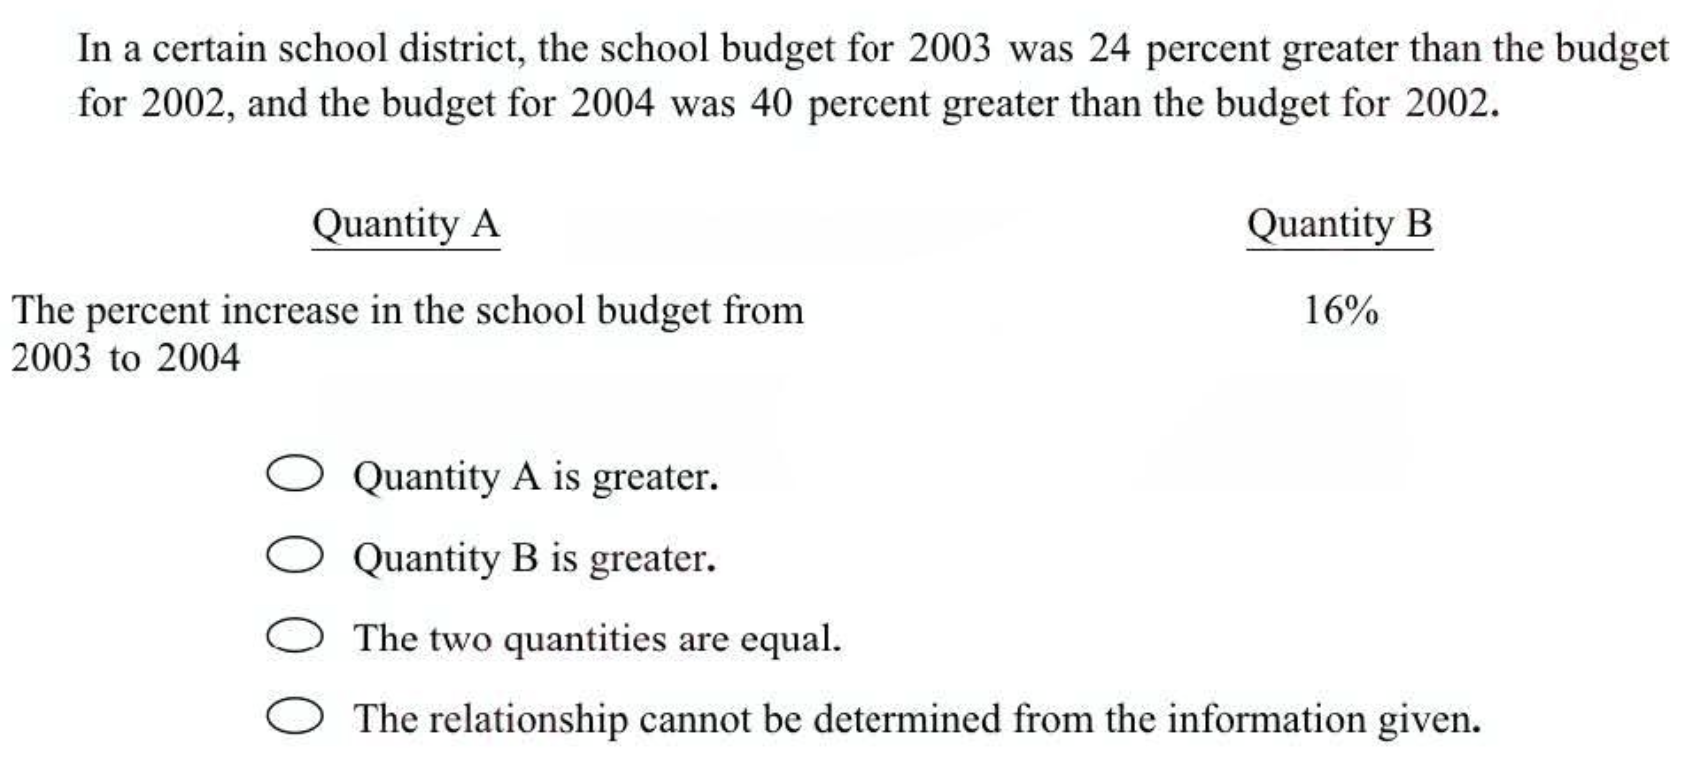
\includegraphics[width=\linewidth]{Percent_Increase_Example_Question1.png}
% 		\caption{-Sec-}
% 	\end{figure}
% 	\pause
% $$ \\
% \pause
% \bigskip
% Answer \textbf{B } 
% \end{frame}

% %------------------------------------------------


%------------------------------------------------

% \begin{frame}
% 	\frametitle{Have a try!}
% 	\framesubtitle{}


% \bigskip
% \pause

% \bigskip
% Answer \textbf{- 2.48\%}
% \end{frame}

% %------------------------------------------------
%------------------------------------------------
% \section{Text Examples} % Sections are added in order to organize your presentation into discrete blocks, all sections and subsections are automatically output to the table of contents as an overview of the talk but NOT output in the presentation as separate slides

% %------------------------------------------------

% \subsection{Paragraphs and Lists}

% \begin{frame}
% 	\frametitle{Paragraphs of Text}
	
% 	Sed iaculis \alert{dapibus gravida}. Morbi sed tortor erat, nec interdum arcu. Sed id lorem lectus. Quisque viverra augue id sem ornare non aliquam nibh tristique. Aenean in ligula nisl. Nulla sed tellus ipsum. Donec vestibulum ligula non lorem vulputate fermentum accumsan neque mollis.
	
% 	\bigskip % Vertical whitespace
	
% 	% Quote example
% 	\begin{quote}
% 		Sed diam enim, sagittis nec condimentum sit amet, ullamcorper sit amet libero. Aliquam vel dui orci, a porta odio.\\
% 		--- Someone, somewhere\ldots
% 	\end{quote}
	
% 	\bigskip % Vertical whitespace
	
% 	Nullam id suscipit ipsum. Aenean lobortis commodo sem, ut commodo leo gravida vitae. Pellentesque vehicula ante iaculis arcu pretium rutrum eget sit amet purus. Integer ornare nulla quis neque ultrices lobortis.
% \end{frame}

% %------------------------------------------------

% \begin{frame}
% 	\frametitle{Lists}
% 	\framesubtitle{Bullet Points and Numbered Lists} % Optional subtitle
	
% 	\begin{itemize}
% 		\item Lorem ipsum dolor sit amet, consectetur adipiscing elit
% 		\item Aliquam blandit faucibus nisi, sit amet dapibus enim tempus
% 		\begin{itemize}
% 			\item Lorem ipsum dolor sit amet, consectetur adipiscing elit
% 			\item Nam cursus est eget velit posuere pellentesque
% 		\end{itemize}
% 		\item Nulla commodo, erat quis gravida posuere, elit lacus lobortis est, quis porttitor odio mauris at libero
% 	\end{itemize}
	
% 	\bigskip % Vertical whitespace
	
% 	\begin{enumerate}
% 		\item Nam cursus est eget velit posuere pellentesque
% 		\item Vestibulum faucibus velit a augue condimentum quis convallis nulla gravida 
% 	\end{enumerate}
% \end{frame}

% %------------------------------------------------

% \subsection{Blocks}

% \begin{frame}
% 	\frametitle{Blocks of Highlighted Text}
	
% 	\begin{block}{Block Title}
% 		Lorem ipsum dolor sit amet, consectetur adipiscing elit. Integer lectus nisl, ultricies in feugiat rutrum, porttitor sit amet augue.
% 	\end{block}
	
% 	\begin{exampleblock}{Example Block Title}
% 		Aliquam ut tortor mauris. Sed volutpat ante purus, quis accumsan.
% 	\end{exampleblock}
	
% 	\begin{alertblock}{Alert Block Title}
% 		Pellentesque sed tellus purus. Class aptent taciti sociosqu ad litora torquent per conubia nostra, per inceptos himenaeos.
% 	\end{alertblock}
	
% 	\begin{block}{} % Block without title
% 		Suspendisse tincidunt sagittis gravida. Curabitur condimentum, enim sed venenatis rutrum, ipsum neque consectetur orci.
% 	\end{block}
% \end{frame}

% %------------------------------------------------

% \subsection{Columns}

% \begin{frame}
% 	\frametitle{Multiple Columns}
% 	\framesubtitle{Subtitle} % Optional subtitle
	
% 	\begin{columns}[t] 
% 		\begin{column}{0.5\textwidth} % Left column width
% 		\end{column}
% 		\begin{column}{0.5\textwidth} % Right column width
% 	\end{columns}





% \end{frame}

% %------------------------------------------------

% \section{Table and Figure Examples}

% \subsection{Table}

% \begin{frame}
% 	\frametitle{Table}
% 	\framesubtitle{Subtitle} % Optional subtitle
	
% 	\begin{table}
% 		\begin{tabular}{l l l}
% 			\toprule
% 			\textbf{Treatments} & \textbf{Response 1} & \textbf{Response 2}\\
% 			\midrule
% 			Treatment 1 & 0.0003262 & 0.562 \\
% 			Treatment 2 & 0.0015681 & 0.910 \\
% 			Treatment 3 & 0.0009271 & 0.296 \\
% 			\bottomrule
% 		\end{tabular}
% 		\caption{Table caption}
% 	\end{table}
% \end{frame}

% %------------------------------------------------

% \subsection{Figure}

% \begin{frame}
% 	\frametitle{Figure}
	
% 	\begin{figure}
% 		
\includegraphics[width=0.8\linewidth]{creodocs_logo.pdf}
% 		\caption{Creodocs logo.}
% 	\end{figure}





% \end{frame}

% %------------------------------------------------

% \section{Mathematics}

% \begin{frame}
% 	\frametitle{Definitions \& Examples}
	
% 	\begin{definition}
% 		A \alert{prime number} is a number that has exactly two divisors.
% 	\end{definition}
	
% 	\smallskip % Vertical whitespace
	
% 	\begin{example}
% 		\begin{itemize}
% 			\item 2 is prime (two divisors: 1 and 2).
% 			\item 3 is prime (two divisors: 1 and 3).
% 			\item 4 is not prime (\alert{three} divisors: 1, 2, and 4).
% 		\end{itemize}
% 	\end{example}
	
% 	\smallskip % Vertical whitespace
	
% 	You can also use the \texttt{theorem}, \texttt{lemma}, \texttt{proof} and \texttt{corollary} environments.
% \end{frame}

% %------------------------------------------------

% \begin{frame}
% 	\frametitle{Theorem, Corollary \& Proof}
	
% 	\begin{theorem}[Mass--energy equivalence]
% 		$E = mc^2$
% 	\end{theorem}
	
% 	\begin{corollary}
% 		$x + y = y + x$
% 	\end{corollary}
	
% 	\begin{proof}
% 		$\omega + \phi = \epsilon$
% 	\end{proof}
% \end{frame}

% %------------------------------------------------

% \begin{frame}
% 	\frametitle{Equation}

% 	\begin{equation}
% 		\cos^3 \theta =\frac{1}{4}\cos\theta+\frac{3}{4}\cos 3\theta
% 	\end{equation}
% \end{frame}

% %------------------------------------------------

% \begin{frame}[fragile] % Need to use the fragile option when verbatim is used in the slide
% 	\frametitle{Verbatim}
	
% 	\begin{example}[Theorem Slide Code]
% 		\begin{verbatim}
% 			\begin{frame}
% 				\frametitle{Theorem}
% 				\begin{theorem}[Mass--energy equivalence]
% 					$E = mc^2$
% 				\end{theorem}
% 		\end{frame}\end{verbatim} % Must be on the same line
% 	\end{example}
% \end{frame}

% %------------------------------------------------

% \begin{frame}
% 	Slide without title.
% \end{frame}

% %------------------------------------------------

% \section{Referencing}

% \begin{frame}
% 	\frametitle{Citing References}
	
% 	An example of the \texttt{\textbackslash cite} command to cite within the presentation:
	
% 	\bigskip % Vertical whitespace
	
% 	This statement requires citation \cite{p1,p2}.
% \end{frame}

% %------------------------------------------------

% \begin{frame} % Use [allowframebreaks] to allow automatic splitting across slides if the content is too long
% 	\frametitle{References}
	
% 	\begin{thebibliography}{99} % Beamer does not support BibTeX so references must be inserted manually as below, you may need to use multiple columns and/or reduce the font size further if you have many references
% 		\footnotesize % Reduce the font size in the bibliography
		
% 		\bibitem[Smith, 2022]{p1}
% 			John Smith (2022)
% 			\newblock Publication title
% 			\newblock \emph{Journal Name} 12(3), 45 -- 678.
			
% 		\bibitem[Kennedy, 2023]{p2}
% 			Annabelle Kennedy (2023)
% 			\newblock Publication title
% 			\newblock \emph{Journal Name} 12(3), 45 -- 678.
% 	\end{thebibliography}
% \end{frame}

% %----------------------------------------------------------------------------------------
% %	ACKNOWLEDGMENTS SLIDE
% %----------------------------------------------------------------------------------------

% \begin{frame}
% 	\frametitle{Acknowledgements}
	
% 	\begin{columns}[t] % The "c" option specifies centered vertical alignment while the "t" option is used for top vertical alignment
% 		\begin{column}{0.45\textwidth} % Left column width
% 			\textbf{Smith Lab}
% 			\begin{itemize}
% 				\item Alice Smith
% 				\item Devon Brown
% 			\end{itemize}
% 			\textbf{Cook Lab}
% 			\begin{itemize}
% 				\item Margaret
% 				\item Jennifer
% 				\item Yuan
% 			\end{itemize}
% 		\end{column}		
% 		\begin{column}{0.5\textwidth} % Right column width
% 			\textbf{Funding}
% 			\begin{itemize}
% 				\item British Royal Navy
% 				\item Norwegian Government
% 			\end{itemize}
% 		\end{column}
% 	\end{columns}
% \end{frame}

%----------------------------------------------------------------------------------------
%	CLOSING SLIDE
%----------------------------------------------------------------------------------------

\begin{frame}[plain] % The optional argument 'plain' hides the headline and footline
	\begin{center}
		{\Huge 1 Min Break}
		\bigskip\bigskip % Vertical whitespace
		
		{\LARGE Questions? Comments?}
	\end{center}
\end{frame}

%----------------------------------------------------------------------------------------

\end{document} 